\clearpage

\part{Predictions, Discussion, and Conclusion}
  \label{part:predictions-discussion-and-conclusion}

  This final part collects the phenomenological consequences of the Cosmochrony framework and
  confronts them with observation.
  Radiation processes, mass spectra, and quantization effects are revisited from a unified
  structural perspective, leading to concrete and falsifiable predictions.

  Testable signatures are identified across cosmology, gravitation, particle physics, and
  high-energy regimes, with particular attention to discriminating Cosmochrony from
  $\Lambda$CDM-based models and standard quantum-gravitational extensions.

  The concluding discussion situates Cosmochrony with respect to existing theoretical
  frameworks, clarifies its domain of validity, and highlights open challenges.
  Rather than proposing a final theory, this part frames Cosmochrony as a coherent
  pre-geometric research program constrained by internal consistency and empirical
  accessibility.

  \clearpage
  \clearpage

\section{Radiation and Quantization}
\label{sec:radiation-and-quantization}

% ----------------------------------------------------------------------------
% Section 9.1 --- Radiation as chi--Matter Interaction
% From former §13.1, condensed
% ----------------------------------------------------------------------------
\subsection{Radiation as
\texorpdfstring{$\chi$}{χ}--Matter Interaction}
\label{subsec:radiation-as-chimatter-interaction}

Radiation arises when a localized, relaxation-resistant configuration
undergoes a transition toward a less constrained state.
The excess relational content ceases to admit a particle-like projected
description and becomes expressible only through delocalized projected
modes.
In effective spacetime descriptions, this redistribution appears as
radiative emission---a transfer of descriptive weight from particle-like
configurations to propagating field-like descriptions, without invoking
discrete objects or stochastic processes.

% ----------------------------------------------------------------------------
% Section 9.2 --- Emergence of Photons
% From former §13.2, condensed
% ----------------------------------------------------------------------------
\subsection{Emergence of Photons}
\label{subsec:emergence-of-photons}

Photons are not fundamental entities.
Prior to emission or detection, no photon exists as an independent
object.
A reconfiguration of relational structure within~$\chi$ ceases to admit
a localized projection and becomes expressible only through extended,
delocalized effective modes---represented in spacetime as electromagnetic
waves.

Photon-like events emerge only at interaction: when a delocalized
projective mode becomes locally constrained by interaction with a
localized excitation, the projection resolves into a discrete transfer of
relaxation capacity.
Quantization is a property of interaction and local reprojection, not of
propagation.
Wave--particle duality reflects a duality of description rather than of
underlying ontology.
Interference phenomena arise from the coherence of delocalized projective
modes; individual detection events correspond to localized reprojections.

% ----------------------------------------------------------------------------
% Section 4.5 --- Energy--Frequency Relation
% From former §6.5
% ----------------------------------------------------------------------------
\subsection{Energy--Frequency Relation}
\label{subsec:energy-frequency-solitons}

The energy associated with a particle-like excitation is linked to a
characteristic internal spectral scale of the corresponding projected
configuration.
Configurations associated with higher characteristic frequencies
correspond to more tightly constrained structures and encode greater
effective resistance to relaxation.
This yields
\begin{equation}
  E \propto \nu ,
\end{equation}
where $\nu$ characterizes the spectral scale of internal organization.
Planck's constant appears as an effective proportionality factor whose
universality reflects the robustness of spectral scales in the current
relaxation epoch.
A more explicit realization in the context of radiation is presented in
Section~\ref{subsec:energy-frequency-radiation}.

% ----------------------------------------------------------------------------
% Section 9.4 --- Vacuum Fluctuations and the Casimir Effect
% From former §13.4, condensed
% ----------------------------------------------------------------------------
\subsection{Vacuum Fluctuations and the Casimir Effect}
\label{subsec:vacuum-fluctuations-and-the-casimir-effect}

Vacuum fluctuations reflect the intrinsic structural indeterminacy
of~$\chi$ in regimes where no stable localized excitations are present.
The relaxation admits a wide range of locally compatible projective
descriptions; these fluctuations represent variability of effective
descriptions rather than physical energy stored in the vacuum.

When material boundaries impose structural constraints on local
projectability, certain effective descriptions become incompatible with
the boundary conditions, reducing the set of admissible projective
configurations between the boundaries.
The Casimir effect arises from this asymmetry: a difference in the
density of admissible effective reprojections, manifesting as a pressure
on the confining surfaces.
No fundamental vacuum energy density or propagating vacuum modes are
required.

% ----------------------------------------------------------------------------
% Section 9.5 --- Weakly Interacting Radiation
% From former §13.5, condensed
% ----------------------------------------------------------------------------
\subsection{Weakly Interacting Radiation}
\label{subsec:weakly-interacting-radiation}

Weakly interacting radiation corresponds to delocalized projective
regimes whose structural contrast is insufficient to efficiently induce
localized reprojection upon encountering matter.
Low-frequency or weakly coupled modes are characterized by smooth, slowly
varying relational structure, strongly suppressing the probability of
stable localized energy transfer.
Small interaction cross sections reflect the low likelihood that a given
projective configuration satisfies the geometric and topological
conditions required for localized reprojection.

\input{5-predictions_discussion_and_conclusion/09-radiation-and-quantization/sec-summary-radiation}

  \clearpage

\section{Radiation and Quantization}
\label{sec:radiation-and-quantization}

% ----------------------------------------------------------------------------
% Section 9.1 --- Radiation as chi--Matter Interaction
% From former §13.1, condensed
% ----------------------------------------------------------------------------
\subsection{Radiation as
\texorpdfstring{$\chi$}{χ}--Matter Interaction}
\label{subsec:radiation-as-chimatter-interaction}

Radiation arises when a localized, relaxation-resistant configuration
undergoes a transition toward a less constrained state.
The excess relational content ceases to admit a particle-like projected
description and becomes expressible only through delocalized projected
modes.
In effective spacetime descriptions, this redistribution appears as
radiative emission---a transfer of descriptive weight from particle-like
configurations to propagating field-like descriptions, without invoking
discrete objects or stochastic processes.

% ----------------------------------------------------------------------------
% Section 9.2 --- Emergence of Photons
% From former §13.2, condensed
% ----------------------------------------------------------------------------
\subsection{Emergence of Photons}
\label{subsec:emergence-of-photons}

Photons are not fundamental entities.
Prior to emission or detection, no photon exists as an independent
object.
A reconfiguration of relational structure within~$\chi$ ceases to admit
a localized projection and becomes expressible only through extended,
delocalized effective modes---represented in spacetime as electromagnetic
waves.

Photon-like events emerge only at interaction: when a delocalized
projective mode becomes locally constrained by interaction with a
localized excitation, the projection resolves into a discrete transfer of
relaxation capacity.
Quantization is a property of interaction and local reprojection, not of
propagation.
Wave--particle duality reflects a duality of description rather than of
underlying ontology.
Interference phenomena arise from the coherence of delocalized projective
modes; individual detection events correspond to localized reprojections.

% ----------------------------------------------------------------------------
% Section 4.5 --- Energy--Frequency Relation
% From former §6.5
% ----------------------------------------------------------------------------
\subsection{Energy--Frequency Relation}
\label{subsec:energy-frequency-solitons}

The energy associated with a particle-like excitation is linked to a
characteristic internal spectral scale of the corresponding projected
configuration.
Configurations associated with higher characteristic frequencies
correspond to more tightly constrained structures and encode greater
effective resistance to relaxation.
This yields
\begin{equation}
  E \propto \nu ,
\end{equation}
where $\nu$ characterizes the spectral scale of internal organization.
Planck's constant appears as an effective proportionality factor whose
universality reflects the robustness of spectral scales in the current
relaxation epoch.
A more explicit realization in the context of radiation is presented in
Section~\ref{subsec:energy-frequency-radiation}.

% ----------------------------------------------------------------------------
% Section 9.4 --- Vacuum Fluctuations and the Casimir Effect
% From former §13.4, condensed
% ----------------------------------------------------------------------------
\subsection{Vacuum Fluctuations and the Casimir Effect}
\label{subsec:vacuum-fluctuations-and-the-casimir-effect}

Vacuum fluctuations reflect the intrinsic structural indeterminacy
of~$\chi$ in regimes where no stable localized excitations are present.
The relaxation admits a wide range of locally compatible projective
descriptions; these fluctuations represent variability of effective
descriptions rather than physical energy stored in the vacuum.

When material boundaries impose structural constraints on local
projectability, certain effective descriptions become incompatible with
the boundary conditions, reducing the set of admissible projective
configurations between the boundaries.
The Casimir effect arises from this asymmetry: a difference in the
density of admissible effective reprojections, manifesting as a pressure
on the confining surfaces.
No fundamental vacuum energy density or propagating vacuum modes are
required.

% ----------------------------------------------------------------------------
% Section 9.5 --- Weakly Interacting Radiation
% From former §13.5, condensed
% ----------------------------------------------------------------------------
\subsection{Weakly Interacting Radiation}
\label{subsec:weakly-interacting-radiation}

Weakly interacting radiation corresponds to delocalized projective
regimes whose structural contrast is insufficient to efficiently induce
localized reprojection upon encountering matter.
Low-frequency or weakly coupled modes are characterized by smooth, slowly
varying relational structure, strongly suppressing the probability of
stable localized energy transfer.
Small interaction cross sections reflect the low likelihood that a given
projective configuration satisfies the geometric and topological
conditions required for localized reprojection.

\input{5-predictions_discussion_and_conclusion/09-radiation-and-quantization/sec-summary-radiation}

  \clearpage

\section{Radiation and Quantization}
\label{sec:radiation-and-quantization}

% ----------------------------------------------------------------------------
% Section 9.1 --- Radiation as chi--Matter Interaction
% From former §13.1, condensed
% ----------------------------------------------------------------------------
\subsection{Radiation as
\texorpdfstring{$\chi$}{χ}--Matter Interaction}
\label{subsec:radiation-as-chimatter-interaction}

Radiation arises when a localized, relaxation-resistant configuration
undergoes a transition toward a less constrained state.
The excess relational content ceases to admit a particle-like projected
description and becomes expressible only through delocalized projected
modes.
In effective spacetime descriptions, this redistribution appears as
radiative emission---a transfer of descriptive weight from particle-like
configurations to propagating field-like descriptions, without invoking
discrete objects or stochastic processes.

% ----------------------------------------------------------------------------
% Section 9.2 --- Emergence of Photons
% From former §13.2, condensed
% ----------------------------------------------------------------------------
\subsection{Emergence of Photons}
\label{subsec:emergence-of-photons}

Photons are not fundamental entities.
Prior to emission or detection, no photon exists as an independent
object.
A reconfiguration of relational structure within~$\chi$ ceases to admit
a localized projection and becomes expressible only through extended,
delocalized effective modes---represented in spacetime as electromagnetic
waves.

Photon-like events emerge only at interaction: when a delocalized
projective mode becomes locally constrained by interaction with a
localized excitation, the projection resolves into a discrete transfer of
relaxation capacity.
Quantization is a property of interaction and local reprojection, not of
propagation.
Wave--particle duality reflects a duality of description rather than of
underlying ontology.
Interference phenomena arise from the coherence of delocalized projective
modes; individual detection events correspond to localized reprojections.

% ----------------------------------------------------------------------------
% Section 4.5 --- Energy--Frequency Relation
% From former §6.5
% ----------------------------------------------------------------------------
\subsection{Energy--Frequency Relation}
\label{subsec:energy-frequency-solitons}

The energy associated with a particle-like excitation is linked to a
characteristic internal spectral scale of the corresponding projected
configuration.
Configurations associated with higher characteristic frequencies
correspond to more tightly constrained structures and encode greater
effective resistance to relaxation.
This yields
\begin{equation}
  E \propto \nu ,
\end{equation}
where $\nu$ characterizes the spectral scale of internal organization.
Planck's constant appears as an effective proportionality factor whose
universality reflects the robustness of spectral scales in the current
relaxation epoch.
A more explicit realization in the context of radiation is presented in
Section~\ref{subsec:energy-frequency-radiation}.

% ----------------------------------------------------------------------------
% Section 9.4 --- Vacuum Fluctuations and the Casimir Effect
% From former §13.4, condensed
% ----------------------------------------------------------------------------
\subsection{Vacuum Fluctuations and the Casimir Effect}
\label{subsec:vacuum-fluctuations-and-the-casimir-effect}

Vacuum fluctuations reflect the intrinsic structural indeterminacy
of~$\chi$ in regimes where no stable localized excitations are present.
The relaxation admits a wide range of locally compatible projective
descriptions; these fluctuations represent variability of effective
descriptions rather than physical energy stored in the vacuum.

When material boundaries impose structural constraints on local
projectability, certain effective descriptions become incompatible with
the boundary conditions, reducing the set of admissible projective
configurations between the boundaries.
The Casimir effect arises from this asymmetry: a difference in the
density of admissible effective reprojections, manifesting as a pressure
on the confining surfaces.
No fundamental vacuum energy density or propagating vacuum modes are
required.

% ----------------------------------------------------------------------------
% Section 9.5 --- Weakly Interacting Radiation
% From former §13.5, condensed
% ----------------------------------------------------------------------------
\subsection{Weakly Interacting Radiation}
\label{subsec:weakly-interacting-radiation}

Weakly interacting radiation corresponds to delocalized projective
regimes whose structural contrast is insufficient to efficiently induce
localized reprojection upon encountering matter.
Low-frequency or weakly coupled modes are characterized by smooth, slowly
varying relational structure, strongly suppressing the probability of
stable localized energy transfer.
Small interaction cross sections reflect the low likelihood that a given
projective configuration satisfies the geometric and topological
conditions required for localized reprojection.

\input{5-predictions_discussion_and_conclusion/09-radiation-and-quantization/sec-summary-radiation}

  \clearpage

\section{Discussion and Comparison with Existing Frameworks}
\label{sec:discussion-and-comparison-with-existing-frameworks}

\subsection{Relation to General Relativity}
\label{subsec:relation-to-general-relativity}

Spacetime curvature in Cosmochrony is an emergent descriptive construct
(Section~\ref{subsec:emergent-curvature}).
No \emph{a priori} metric dynamics is postulated; instead, an effective
geometry emerges from variations in local relaxation dynamics.
Matter configurations locally constrain the relaxation of~$\chi$,
leading to differential rates of effective proper-time evolution that are
reinterpreted as effective metric deformations.
In the weak-field regime, Newtonian gravity is reproduced; in the
strong-field limit, Schwarzschild-like solutions emerge.
General Relativity is recovered as the appropriate effective theory
within its empirically validated domain.

% ----------------------------------------------------------------------------
% Section 12.2 --- Relation to Quantum Formalism
% From former §15.2, condensed
% ----------------------------------------------------------------------------
\subsection{Relation to Quantum Formalism}
\label{subsec:relation-to-quantum-formalism}

Cosmochrony does not treat quantization or wave dynamics as
fundamental~\cite{PeskinSchroeder1995QFT}.
Particles correspond to localized, topologically stable configurations;
discrete observables arise from boundary conditions, topological
constraints, and interaction-induced reprojection.
The Planck relation $E = h\nu$ is a geometric correspondence between
redistributed relaxation potential and minimal projective resolution.
Entanglement reflects a shared, non-factorizable~$\chi$ configuration
persisting only within a finite critical regime of projection, while
decoherence reflects irreversible loss of relational accessibility.

\subsection{Analogy with Collective Phenomena in QCD}
  \label{subsec:analogy-with-collective-phenomena-in-qcd}

  A useful structural analogy may be drawn with low-energy
  QCD~\cite{Shifman2007QCDVacuum}, where fundamental degrees of freedom
  (quarks, gluons) do not appear as isolated entities in the infrared.
  The observable spectrum consists instead of collective bound states,
  whose properties are not transparently reducible to perturbative
  constituents.

  Similarly, Cosmochrony formulates fundamental dynamics solely in terms
  of~$\chi$ and its relaxation ordering.
  Observable quantities arise only after projection into regimes
  admitting stable effective descriptions.
  What appear as elementary constituents at a given effective level may
  represent stable, regime-dependent invariants of the underlying
  dynamics, in direct analogy with QCD confinement.

  The analogy extends beyond particle confinement.
  In QCD, the vacuum itself admits multiple collective phases,
  including chiral symmetry breaking and color superconductivity,
  which emerge from non-perturbative organization of the same
  underlying degrees of freedom.
  In Cosmochrony, different physical phenomena likewise correspond
  to distinct collective regimes of a single substrate.

  Gravitational curvature arises as a collective slowdown of relaxation
  ordering.
  Schwinger pair production corresponds to saturation of directed
  relaxation flux.
  Superconductivity, as discussed in
  Section~\ref{subsec:collective-U1-coherence},
  represents a coherent collective phase of the $U(1)$ fiber sector,
  in which composite winding classes stabilize and lock globally.

  In all these cases, the effective phenomena are not introduced
  as additional dynamical postulates.
  They correspond to regime-dependent reorganizations of the same
  projective structure.
  The underlying ontology remains unchanged, while the effective
  description undergoes phase-like transitions analogous to those
  observed in strongly coupled gauge theories.

  This analogy is structural rather than dynamical.
  Cosmochrony does not import the specific field content of QCD.
  The comparison serves to clarify how radically different effective
  laws may arise from a single underlying relational dynamics,
  without multiplying fundamental entities.

% ----------------------------------------------------------------------------
% Section 12.4 --- Comparison with ΛCDM Cosmology
% From former §15.4, condensed
% ----------------------------------------------------------------------------
\subsection{Comparison with
\texorpdfstring{$\Lambda$}{Λ}CDM Cosmology}
\label{subsec:comparison-with-lambdacdm-cosmology}

$\Lambda$CDM introduces cold dark matter, dark energy, and inflation as
effective
postulates~\cite{peebles1993principles,planck2020results}.
In Cosmochrony, cosmic expansion follows from monotonic relaxation of
the substrate, with $H(t) = \dot{\chi}/\chi$ and
$H_0 \sim c/\chi(t_0)$.
Dark energy is reinterpreted as the large-scale relaxation dynamics;
cosmic acceleration reflects cumulative relaxation over cosmological
timescales.
The coincidence problem and the Hubble tension may admit interpretations
in terms of epoch-dependent relaxation dynamics rather than new
fundamental constituents.
Low-$\ell$ CMB suppression is explored as a structural consequence of
relaxation constraints rather than a statistical fluctuation.

Table~\ref{tab:comparison_cosmochrony} summarizes the conceptual
differences between Cosmochrony, $\Lambda$CDM, and Loop Quantum Gravity.

% ----------------------------------------------------------------------------
% Section 12.5 --- Historical Admissibility
% From former §15.5, condensed
% ----------------------------------------------------------------------------
\subsection{Historical Admissibility of Projected Degrees of Freedom}
\label{subsec:historical-admissibility}

The set of effective degrees of freedom depends on the admissibility
conditions imposed by the relaxation state.
In the early Universe, only highly coherent, low-complexity global
configurations were admissible.
As relaxation proceeds, the admissible space progressively enlarges,
enabling increasingly localized invariants described as particles,
fields, and interactions.
The particle spectrum is therefore a historically conditioned outcome of
relaxation dynamics, not a timeless feature.
This perspective reconciles the emergence of complexity with monotonic
entropy increase: the early Universe is characterized by both low entropy
and low admissible complexity.
Low-$\ell$ CMB anomalies may be interpreted as relics of this early
regime of restricted admissibility.

\subsection{Inflation, Horizon Problems, and Initial Conditions}
\label{subsec:inflation-horizon-problems-and-initial-conditions}

Because~$\chi$ describes a global relaxation process rather than metric
expansion, causal connectivity is not defined in terms of spacetime
lightcones at the fundamental level.
Large-scale coherence arises from initial relational smoothness and
subsequent monotonic relaxation, without requiring an inflationary phase.
The horizon problem is rendered inoperative by the absence of an
initially fragmented causal structure at the pre-geometric level.
A detailed quantitative treatment of primordial perturbations and their
CMB imprint remains an open direction for future work.

% ----------------------------------------------------------------------------
% Section 12.7 --- Conceptual Implications and Open Challenges
% From former §15.7, condensed
% ----------------------------------------------------------------------------
\subsection{Conceptual Implications and Open Challenges}
\label{subsec:conceptual-implications-and-open-challenges}

Temporal ordering arises from the monotonic relaxation of~$\chi$; energy
quantifies residual capacity to resist this relaxation; irreversibility
reflects its progressive exhaustion.
Time, energy, and irreversibility are not independent axioms but
complementary effective descriptions of the same relational dynamics.

Open challenges include the quantitative reconstruction of CMB
anisotropies from early-time $\chi$ dynamics, the detailed treatment of
non-equilibrium decoherence and reprojection, the emergence of gauge
symmetries from topological features, and the long-term stability of
solitonic configurations under extreme conditions.
Progress will require large-scale simulations of $\chi$ dynamics,
discretized lattice realizations, and targeted experimental tests.

\input{5-predictions_discussion_and_conclusion/12-discussion-and-comparison-with-existing-frameworks/008-ontological-parsimony}
\subsection{Relation to the Higgs Mechanism: Emergence from
\texorpdfstring{$\chi$}{χ} Dynamics}
  \label{subsec:relation-to-the-higgs-mechanism}

  The Higgs field and its VEV are reinterpreted as effective low-energy
  descriptors of a specific projective regime of~$\chi$.

  \subsubsection*{Structural Transition}
    \label{subsec:emergence-higgs-vev}
    \label{subsec:chi_c-electroweak-scale}
    Below a critical scale~$\chi_c$ (homogeneous regime), only massless
    globally coherent configurations are admissible.
    Above~$\chi_c$ (structured regime), localized relaxation-resistant
    configurations stabilize as massive excitations.
    The electroweak scale is related through
    \begin{equation}
      \langle \phi_H \rangle
      \;\propto\;
      \frac{\hbar_{\mathrm{eff}}\, c}{\chi_c},
    \end{equation}
    naturally recovering the observed scale for $\chi_c \sim 10^{-18}\,\mathrm{m}$.

  \subsubsection*{Mass Generation as Solitonic Stabilization}
    \label{subsec:mass-generation-solitons}
    Fermion masses scale as
    $m_f \propto y_f\,\hbar_{\mathrm{eff}}/\chi_c$;
    gauge boson masses as
    $m_W \propto g\,\hbar_{\mathrm{eff}}/\chi_c$.
    These relations reproduce standard Higgs-generated mass terms at the effective level.

    Within the spectral interpretation developed in Section~\ref{subsec:flavor-structure-cp},
    the Yukawa parameters encode the effective projection of underlying relaxation eigenvalues.
    The observed flavor hierarchies and associated CP structure therefore reflect the same spectral organization,
    rather than introducing independent mass-generating dynamics.

    Within the spectral interpretation developed in Section~\ref{subsec:flavor-structure-cp},
    the Yukawa parameters encode the effective projection of underlying relaxation eigenvalues.
    The observed flavor hierarchies and associated CP structure therefore reflect the same spectral organization,
    rather than introducing independent mass-generating dynamics.

  \subsubsection*{Phenomenological Status}
    \label{subsec:phenomenological-implications}
    \label{subsec:higgs-summary}
    No deviation from established collider results is implied at accessible energies.
    Departures may arise only in extreme regimes.
    Open challenges include deriving the detailed mapping between~$\chi$
    soliton spectra and the full Standard Model mass spectrum.

% ----------------------------------------------------------------------------
% Section 12.10 --- Structural Interpretation: Projective Thermodynamics
% From former §15.10, condensed
% ----------------------------------------------------------------------------
\subsection{Structural Interpretation: Projective Thermodynamics}
\label{subsec:structural-interpretation-projective-thermodynamics}

Physical observables arise through a generically non-injective projection
$\Pi : \Omega \rightarrow O$.
In saturation regimes, the resulting loss of distinguishability induces a
structural entropy:
\begin{equation}
  S_{\Pi} = -\sum_{o \in O}
    \mu(\Pi^{-1}(o)) \log \mu(\Pi^{-1}(o)),
\end{equation}
which is an objective property of the projection.

\begin{figure}[t]
  \centering
  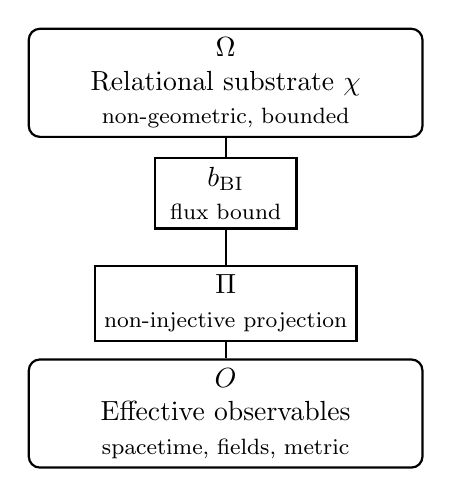
\begin{tikzpicture}[
    node distance=1.4cm,
    every node/.style={align=center},
    box/.style={draw, rounded corners, thick,
      minimum width=5cm, minimum height=1cm},
    narrow/.style={draw, thick,
      minimum width=1.8cm, minimum height=0.8cm}
  ]
    \node[box] (omega)
      {$\Omega$\\Relational substrate $\chi$\\
       {\footnotesize non-geometric, bounded}};
    \node[narrow, below of=omega] (bi)
      {$b_{\mathrm{BI}}$\\
       {\footnotesize flux bound}};
    \node[narrow, below of=bi] (pi)
      {$\Pi$\\
       {\footnotesize non-injective projection}};
    \node[box, below of=pi] (obs)
      {$O$\\Effective observables\\
       {\footnotesize spacetime, fields, metric}};
    \draw[thick] (omega) -- (bi);
    \draw[thick] (bi) -- (pi);
    \draw[thick] (pi) -- (obs);
  \end{tikzpicture}
  \caption{Projective regimes in Cosmochrony.
    The substrate~$\Omega$ undergoes bounded relaxation
    ($b_{\mathrm{BI}}$).
    Observables arise through non-injective projection~$\Pi$.}
  \label{fig:projective-hourglass}
\end{figure}

Effective parameters such as temperature or metric curvature emerge as
Lagrange multipliers absorbing unresolved relational complexity.
High effective temperatures or anomalous geometric features reflect the
compression of a bounded relational flux into a reduced observable
description, not excess local energy density.
The bounded character of substratic relaxation ensures that
projection-induced quantities remain finite, rendering the framework
predictive despite the non-injective nature of the projection.

\subsection{Bounds on Projective Resolvability Across Scales}
  \label{subsec:projective-resolvability-bound}

  Saturation phenomena across scales---bounded gravitational response in low-density environments and the operational
  accessibility of quantum correlations---reflect a common limitation on projective resolvability.
  In Cosmochrony, the projected description $U$ does not expose the full relational content of the substrate~$\chi$.
  It exposes only what can be rendered operationally accessible through the non-injective mapping~$\Pi$ under admissible
  update transport.
  The relevant limitation is therefore not a postulated geometric cutoff, but a throughput bound on the rate at which
  relational structure can be updated while maintaining operational closure of the projected state.

  Attosecond chronoscopy experiments illustrate this principle.
  Measured delays can be interpreted as the minimal temporal resolution required for a non-factorizable projected
  description to become operationally resolvable, rather than as a dynamical buildup of correlations~\cite{PhysRevLett.133.163201}.

  We summarize this limitation by an effective inequality on projected update rates,
  \begin{equation}
    \left| \frac{\partial \mathcal{O}_{\mathrm{eff}}}{\partial \tau} \right|
    \;\leq\;
    b_{\chi}\,\mathcal{S}_{\Pi},
    \label{eq:resolvability_bound}
  \end{equation}
  where $b_{\chi}$ is the invariant bound on admissible relaxation transport in the substrate and $\mathcal{S}_{\Pi}$
  parametrizes the effective structural complexity of the projection for the class of observables under consideration.
  The factor $\mathcal{S}_{\Pi}$ is not a new dynamical field.
  It encodes how many independent relational channels can be synchronized within one operational update step.

  Distinct phenomenological manifestations correspond to distinct choices of $\mathcal{O}_{\mathrm{eff}}$ and the associated
  resolution scale.
  In macroscopic weak-field regimes, the same bound induces an operational saturation threshold that can be expressed as an
  effective acceleration proxy,
  \begin{equation}
    a_{\star} \sim \kappa \frac{b_{\chi}}{\ell},
    \label{eq:a_star_b_relation}
  \end{equation}
  where $\ell$ is the local descriptive resolution of the projected state and $\kappa=\mathcal{O}(1)$ encodes the
  normalization convention of~$\Pi$.
  In measurement-limited quantum protocols, the bound similarly appears as a bandwidth constraint,
  \begin{equation}
    B_{\Pi}(\mathcal{M})
    = \eta_{\mathcal{M}}\,b_{\chi}\,\mathcal{S}_{\Pi},
    \label{eq:bandwidth_b_relation}
  \end{equation}
  for a measurement procedure~$\mathcal{M}$, with $\eta_{\mathcal{M}}$ absorbing protocol-dependent conventions.
  These expressions represent different dimensional projections of the same underlying transport bound.
  A modification of the effective resolvability of the $\chi \rightarrow \Pi$ mapping would therefore induce correlated
  shifts in both galactic saturation scales and quantum chronoscopy thresholds.

  A further generic consequence is the divergence of projective stress under sufficiently deep refinement.
  Let $D$ denote an operational update demand, defined as a characteristic rate at which projected relations must be
  recomputed to preserve admissibility.
  Let $C$ denote the admissible projective throughput under the bound~$b_{\chi}$ for the same class of updates.
  The dimensionless stress ratio
  \begin{equation}
    \Xi \equiv \frac{D}{C}
  \end{equation}
  provides a regime indicator.
  Whenever a process increases $D$ faster than $C$ can be redistributed by the available synchronized channels, $\Xi$ grows
  and a saturated reconfiguration becomes unavoidable.
  This statement is independent of any particular emergent geometry and follows solely from bounded transport and finite
  projective resolvability.

\input{5-predictions_discussion_and_conclusion/12-discussion-and-comparison-with-existing-frameworks/012-non-termination}
\input{5-predictions_discussion_and_conclusion/12-discussion-and-comparison-with-existing-frameworks/013-conclusion}

